\documentclass[tikz,border=3pt]{standalone}
\usetikzlibrary{arrows.meta,calc}
\begin{document}
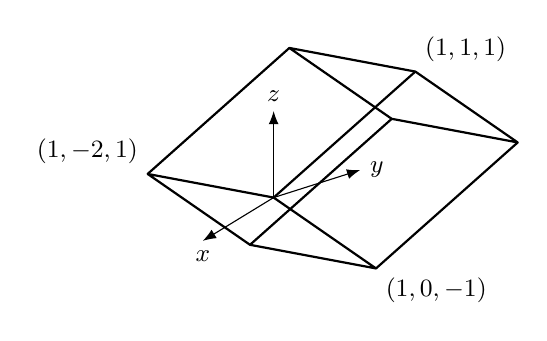
\begin{tikzpicture}[>=Latex, font=\small, line join=round]
  \coordinate (O) at (0,0);
  \coordinate (A) at (-1.6,0.3);
  \coordinate (B) at (1.3,-0.9);
  \coordinate (C) at (1.8,1.6);
  \coordinate (AB) at ($(A)+(B)$);
  \coordinate (AC) at ($(A)+(C)$);
  \coordinate (BC) at ($(B)+(C)$);
  \coordinate (ABC) at ($(A)+(B)+(C)$);

  \draw[thick] (O) -- (A) -- (AB) -- (B) -- cycle;
  \draw[thick] (C) -- (AC) -- (ABC) -- (BC) -- cycle;
  \draw[thick] (O) -- (C);
  \draw[thick] (A) -- (AC);
  \draw[thick] (B) -- (BC);
  \draw[thick] (AB) -- (ABC);

  \draw[->] (O) -- ++(-0.9,-0.55) node[below] {$x$};
  \draw[->] (O) -- ++(1.1,0.35) node[right] {$y$};
  \draw[->] (O) -- ++(0,1.1) node[above] {$z$};

  \node[above left] at (A) {$(1,-2,1)$};
  \node[below right] at (B) {$(1,0,-1)$};
  \node[above right] at (C) {$(1,1,1)$};
\end{tikzpicture}
\end{document}
